%\documentclass{article}
\newcommand{\beginsupplement}{%
        \setcounter{table}{0}
        \renewcommand{\thetable}{S\arabic{table}}%
        \setcounter{figure}{0}
        \renewcommand{\thefigure}{S\arabic{figure}}%
     }
\newcommand{\stopsupplement}{%
        \setcounter{table}{0}
        \renewcommand{\thetable}{\arabic{table}}%
        \setcounter{figure}{0}
        \renewcommand{\thefigure}{\arabic{figure}}%
     }

\documentclass[10pt,twoside,lineno]{gsajnl}
\usepackage{amsmath}
\usepackage[nodisplayskipstretch]{setspace}
\usepackage{makecell} 
\setstretch{1}
% Use the documentclass option 'lineno' to view line numbers

\articletype{preprint} % article type
% {inv} Investigation 
% {gs} Genomic Selection
% {goi} Genetics of Immunity 
% {gos} Genetics of Sex 
% {mp} Multiparental Populations

% adding commenting commands
\newif\ifcomments
\commentstrue
%\commentsfalse
\newcommand{\cjb}[1]{\ifcomments{{\color{blue} \it (#1)}}\else{}\fi}
\newcommand{\plr}[1]{\ifcomments{{\color{purple} \it (#1)}}\else{}\fi}
\newcommand{\ak}[1]{\ifcomments{{\color{red} \it (#1)}}\else{}\fi}


%Space is the Place: How Dispersal and Competition Shape Genetic Variation in Continuous Space
%Impacts of Continuous Spatial Structure on Analyses of Population Genetic Data
%Impacts of Isolation by Distance on Demographic Modeling and Association Studies
%Space is the Place: How Dispersal and Sampling Shape Inference From Genetic Variation in Continuous Space
%Evolution on the Final Frontier: How Dispersal and Sampling Shape Inference From Genetic Data in Continuous Space
\title{Effects of Continuous Spatial Structure on Analysis of Population Genetic Data}

\author[$\ast$,1]{C.J. Battey}
\author[$\ast$]{Peter Ralph}
\author[$\ast$]{Andrew Kern}

\affil[$\ast$]{University of Oregon Dept. Biology, Institute for Ecology Evolution}
\keywords{Space; Population Structure; Demography; Haplotype block sharing; GWAS}

\runningtitle{SPACENESS} % For use in the footer 

%% For the footnote.
%% Give the last name of the first author if only one author;
% \runningauthor{FirstAuthorLastname}
%% last names of both authors if there are two authors;
% \runningauthor{FirstAuthorLastname and SecondAuthorLastname}
%% last name of the first author followed by et al, if more than two authors.
\runningauthor{Battey \textit{et al.}}

\begin{abstract}
Individuals exist in continuous space, but standard models in population genetics are based on discrete randomly-mating populations. As a result many models used to infer selection, phenotypic associations, or past population sizes assume that samples are a random draw from a panmictic population. In reality most populations are structured to some degree across space, but the extent to which this model violation biases common genomic analyses is not well known. Here we implement a forward-time simulation of evolution in continuous space and use it to study the impacts of dispersal and sampling strategy on population genetic summary statistics, demographic inference, and association studies. We find that estimates of past population sizes and many common population genetic summary statistics vary significantly with both dispersal and sampling, with most bias occurring when neighborhood sizes are below 100 and sampling is spatially clustered. Variation in the site frequency spectrum and Tajima's D is greater across sampling strategies than over the range of demographic parameters we simulated, pointing to the need to carefully account for sampling when interpreting results. Last we show that the combination of isolation by distance and spatially correlated environments causes genome-wide signals of association with purely environmental phenotypes in linear-regression GWAS, and that this bias is not fully controlled by regressing out principal components positions during the analysis.  
\end{abstract}

\begin{document}

\maketitle
\thispagestyle{firststyle}
%\marginmark
\firstpagefootnote


\correspondingauthoraffiliation{1}{301 Pacific Hall, University of Oregon Dept. Biology, Institute for Ecology and Evolution. cbattey2@uoregon.edu.}
\vspace{-35pt}% Only used for adjusting extra space in the left column of the first page

\section{Introduction}
The inescapable reality that biological organisms live, move, and reproduce in continuous spatial landscapes has been all but ignored in population genetic models. Indeed, a near universal rule of reproduction is that individuals mate with other nearby individuals, leading to a positive correlation between genetic and geographic distances. This pattern of "isolation by distance" \citep{Wright1943} is one of the most widely replicated empirical findings in population genetics \citep{Chen2017,Jay2012,Sharbel2000}, but classical mathematical models to describing are flawed approximations of the underlying process \citep{Felsenstein1975}.
As a result many studies focus on describing geographic structure as a mixture of random-mating populations connected by migration \citep{Malecot1948,Wright1931}, and analyze variation within clusters of genetic variation inferred by programs like \textit{structure} \citep{Pritchard2000} as random-mating units. 

Though discrete models of between-population differentiation account for much of the genetic variation in species, the assumption that populations are randomly mating at some level has important implications for downstream inference of selection and demography. Methods based on the coalescent \citep{Kingman1982} assume that the sampled individuals are a random draw from a random mating population. If dispersal or mate selection is limited by space these assumptions are violated -- nearby individuals will be more closely related than an average random pair and drawing multiple samples from the same point on the landscape will not represent a random sample of the genetic variation present in the whole population. This is as true at the local scale as it is between the more differentiated units typically analyzed in phylogeographic studies. All downstream inferences drawn from the patterns of relationship inferred among sampled individuals will be subject to bias, but the extent depends on the degree of variation in ancestry across the landscape. 

\ak{we should start by saying that we don't understand how simple summaries will respond to continuous space model}
This issue is particularly important for analyses of polygenic selection, because the allele frequency variation caused by population structure is similar to the pattern expected when many sites in the genome are associated with a given phenotype \citep{Bulik-Sullivan2015}. Indeed two recent studies found that previous evidence of polygenic selection on human height in Europe was badly confounded by population structure \citep{Sohail2018,Berg2018}. As the scale of sequence data now available for many species allows inference of increasingly fine-scale patterns of selection and demography, understanding how and when subtle spatial structure is likely to bias results is an important task for population genetics.

Here we describe an implementation of an individual-based model in continuous space that incorporates overlapping generations, a Gaussian dispersal kernel, and density-dependent fitness. The model scales to chromosome-scale alignments across tens of thousands of individuals, and outputs the full genealogy and recombination history of all final-generation individuals. We use this simulation to test how sampling strategy interacts with isolation by distance to cause systematic variation in population genetic summary statistics typically analyzed under discrete population models. We then examine how the fine-scale spatial structures occurring under limited dispersal impact demographic inference from the site frequency spectrum.

Last we use our model to study the impacts of isolation by distance in continuous space on genome-wide association studies (GWAS). Variation in ancestry proportions between case and control cohorts is expected to cause inflation of test statistics at SNPs with different allele frequencies among populations \citep{Price2006}. Because most phenotypes are influenced by the environment and environmental factors are often spatially correlated, subtle spatial structure within continuous populations can also deflate $p$ values in GWAS of traits influenced by the environment \citep{Mathieson2012}. Here we simulate both the underlying genealogy and phenotypes of a continuously distributed population and seek to identify regions of parameter space -- i.e. the strength of isolation by distance and the spatial distribution of environmental effects on phenotypes -- in which common methods of stratification bias corrections in GWAS are likely to fail. 



\section{Materials and Methods}
\label{sec:materials:methods}

\ak{i moved the following section into M\&M. makes more sense here i think}

\subsection{Modeling Evolution in Continuous Space}
The best-studied approaches to population genetics in continuous space were developed by \cite{Wright1943} and \cite{Malecot1948}, who derived expressions for genetic differentiation in continuous space assuming Poisson distributed numbers of offspring and independent dispersal among individuals. A key finding of Wright's model is that many important aspects of continuous populations can be described in terms of "neighborhood size" -- the number of potential mates for an individual in a given generation, defined as $4\pi\sigma^2d$, where $\sigma$ is the average dispersal distance and $d$ is population density. \cite{Maruyama1972} found that the rate of decline in genetic diversity in a 2-dimensional continuous population approaches the random mating expectation when $d\sigma^2 > 1$, and proposed that this had the important implication that most population genetic expectations for randomly mating populations could be applied to continuously distributed populations with relatively little error. 

Though some aspects of continuous populations are fairly well described by the Wright and Malécot models, \cite{Felsenstein1975} showed that the assumptions of independent dispersal and Poisson distributed offspring that are the basis of these models are incompatible. Over time, a population meeting them will clump into a small number of geographic clusters occupying only a part of the available range. Although real populations are often clumped on landscapes due to factors like varying habitat quality and competition among species, the Wright and Malécot models produce much more extreme clumping than is observed in practice and fail to account for the density-dependent declines in population growth rate that are widely observed in real populations (CITE). 

One method for modeling continuous populations is then to assume the existence of a grid of discrete randomly-mating populations connected by migration, which prevents clustering by forcing all regions to be occupied in every generation. Among many other important results drawn from this class of "lattice" or "stepping stone" models, \cite{Rousset1997} showed that the slope of the a linear regression of genetic differentiation ($F_{st}$) against the logarithm of spatial distance is an estimate of neighborhood size. Though good approximations of continuous structure given high dispersal, these models are not truly continuous, force a uniform realized population density across landscapes, and limit investigation of spatial structure below the level of the deme. An alternative method is to model the geographic spread of ancestry backwards in time through a diffusion approximation -- an approach that has recently made significant progress in modeling both dispersal and demographic parameters \citep{Barton2010,Kelleher2014,Ringbauer2017,Ringbauer2018}.

We took a direct approach to the clustering problem of classical forward-time models by incorporating density dependence into an individual-based model similar to the analytic models developed by Wright and Malécot. By scaling the probability of survival in each timestep to local population density we shift reproductive output towards regions of low-density and prevent populations from clustering. A similar approach was taken previously by \citep{Doebeli2003} who used an individual based model with continuous space and density dependent fitness to study the probability of speciation along continuous environmental gradients. However to our knowledge previous implementations of continuous space models have focused on a small number of genetic loci as the unit of analysis, which limits the ability to investigate the impacts of continuous space on genome-wide genetic variation as is now routinely sampled from real organisms. By simulating chromosome-scale sequence alignments and complete population histories we are able to treat our simulations as real populations and replicate the sampling designs and analyses commonly conducted on real genomic data.
\subsection{A Forward-Time Model of Evolution in Continuous Space}

We implemented our model using the non-Wright-Fisher module in the program SLiM v3.0 \citep{Haller2019}. Each time step consists of three stages: reproduction, dispersal, and competition. To reduce the parameter space we use the same parameter, denoted $\sigma$, to modulate the spatial scale of interactions at all three stages by adjusting the standard deviation of the corresponding Gaussian functions. As in previous work \citep{Wright1943,Ringbauer2017}, $\sigma$ as applied in our dispersal step is approximately equal to the mean parent-offspring distance.  

At the beginning of the simulation individuals are distributed randomly on a continuous landscape. Mates are selected proportional to distances among individuals weighted by a Gaussian function with mean $1/(2\pi\sigma^2)$ and standard deviation $\sigma$. Wright's \cite{Wright1943} "Neighborhood Size", defined as $4\pi\sigma^2 K$ where $K$ is the population density, is then the approximate number of individuals available for mating in our simulation. The number of offspring is drawn from a Poisson distribution with mean $1/L$, where $L$ is the average lifespan. If new offspring are produced, we simulate dispersal by taking two draws from a normal distribution with mean 0 and standard deviation $\sigma$ and adding these to the x and y coordinates of the first parent. 

Density-dependent competition is simulated by adjusting the probability of survival of each individual proportional to the local density of individuals up to a distance $3\sigma$ away, scaled according to the same Gaussian function used for mate selection. Given a per-unit carrying capacity $K$ and average fecundity $F$, the probability of survival $d$ for individual $i$ after adjustment for density is:

\begin{equation}
    d_{i}=min(0.95,\frac{1}{1+\rho*\sum_{i}{G(x)}})
\end{equation}
where 
\begin{equation}
    \rho = F/((1+F)*K)
\end{equation} 
and $G(x)$ is the Gaussian function used to weight distances to other individuals. 

A major challenge in all spatial models is dealing with range edges. When local population density is used to model competition, edge or corner populations can be assigned artificially high fitness values because they lack neighbors within their interaction radius but outside the bounds of the simulation. We approximate a decline in habitat suitability near edges by decreasing the probability of survival proportional to the square root of distance to edges in units of $\sigma$. The final probability of survival for individual \textit{i} is then

\begin{equation}
    s_{i}=d_{i} min(1,\sqrt{x_{i}/\sigma})
    min(1,\sqrt{y_{i}/\sigma})\\
    min(1,\sqrt{(x_{max}-x_{i})/\sigma})
    min(1,\sqrt{(y_{max}-y_{i})/\sigma)}
\end{equation}

where $x$ and $y$ are spatial coordinates. In practice this creates a one $\sigma$ buffer around the edge of the map in which fitness is depressed.

To isolate spatial effects from other components of the model such as overlapping generations, increased variance in reproductive success, and density-dependent fitness, we  also implemented a second version of the SLiM simulation in which mates are selected at random and offspring disperse to a random location on the landscape. We refer to these two models as the "spatial" and "random mating" models. For all simulations the full genealogy and recombination history of final-generation individuals were stored as tree sequences \citep{Kelleher2018}. \ak{add a link to the github repo with code}

We ran 400 simulations for the spatial and random-mating SLiM models on a square landscape of size 50 with per-unit carrying capacity $K=5$ (census $N \approx 10,000$), average lifetime $L=4$, genome size $1\times10^{8}$, recombination rate $1\times10^{-9}$, and drawing $/sigma$ values from a uniform distribution bounded by 0.2 and 4. To speed up the simulations and limit memory overhead we used a mutation rate of 0 in SLiM and later applied mutations to the coalesced tree sequence with msprime's 'mutate( )' function. Because msprime assumes that timesteps are in units of generations, we divided the per-generation rate of $1\times10^{-8} mut/site/gen$ by the generation time estimated for each value of $\sigma$ (see 'Genealogical Parameters' below) to convert the rate to units of mutations/site/timestep. We then verified that this procedure produced the correct number of mutations by comparing a subset of simulations with SLiM-generated mutations (which are applied only at mating events) with mutations added by msprime. Simulations were run for 1.6 million timesteps (approximately 30N generations), or until all extant individuals shared a common ancestor within the simulation (i.e. the tree sequence had coalesced). \ak{maybe worth including a table with some basic runtime results in the supplement?}

\subsection{Genealogical Parameters}
We recorded the census population size and estimated the variance in number of offspring and generation time \ak{need to explain why this is needed} for all simulations. To estimate generation times we stored the age of all parents for 200 timesteps after a 100 generation burn-in and took the mean. To estimate variance in offspring we tracked the number of offspring for all individuals for 100 timesteps following a 100-timestep burn-in period, subset the resulting table to include only the last timestep recorded for each individual, and calculated the variance in number of offspring across all individuals in timesteps 50-100.

\subsection{Sampling}
Our model records the genealogy and sequence variation of the complete population, but in real data genotypes are only observed from a relatively small number of sampled individuals. We modeled three sampling strategies similar to common data collection methods in empirical genetic studies (Figure \ref{fig:samplemap}). "Random" sampling selects individuals at random from across the full landscape, "point" sampling selects individuals proportional to their distance from four equally spaced points on the landscape, and "midpoint" sampling selects individuals in proportion to their distance from the middle of the landscape. Downstream analyses were repeated across all sampling strategies. 

\subsection{Summary Statistics}
We calculated the site frequency spectrum and a set of 18 summary statistics (Supplementary Table \cjb{working on this}) from 60 diploid individuals sampled from the final generation of each simulation using the python package scikit-allel \citep{Miles2017}. Statistics included common single-population summaries including mean pairwise divergence ($\pi$), inbreeding coefficient ($F_{is}$), and Tajima's D, as well as the classic isolation-by-distance regression of genetic distance ($D_{xy}$) against the logarithm of geographic distances \citep{Rousset1997}, which we summarized as the correlation coefficient between $log10(spatial distance)$ and the proportion of identical base pairs among individuals. 

Following recent studies that showed strong signals for dispersal and demography in the distribution of shared haplotype block lengths \citep{Ringbauer2017,Baharian2016}, we also calculated various summaries of the distribution of pairwise identical-by-state (IBS) block lengths among samples. The full distribution of lengths of IBS tracts for each pair of individuals was first calculated with a custom python function \ak{point to code on github}. We then calculated the first three moments of this distribution (mean, variance, and skew) and the number of blocks over $1e6$ base pairs both for each pair of individuals and for the full distribution across all pairwise comparisons. 

We then estimated correlation coefficients between spatial distance and each moment of the pairwise IBS tract distribution. Because more closely related individuals on average share longer haplotype blocks we expect that spatial distance will be negatively correlated with mean haplotype block length, and that this correlation will be strongest (i.e. most negative) when dispersal is low. The variance, skew, and count of long haplotype block statistics are meant to reflect the relative length of the right (upper) tail of the distribution, which represents the frequency of long haplotype blocks so should reflect recent demographic events \citep{Ringbauer2017}. 

The effects of sampling on summary statistic estimates were summarized by testing for differences in mean (ANOVA, \citep{Rcore2018}) and variance (Levene's test, \citep{Fox2011}) across sampling strategies for each summary statistic. 

\subsection{Demographic Modeling}
We fit single-population demographic models to the site frequency spectra of 20 individuals from each spatial SLiM simulation with the program Stairwayplot \citep{Liu2015}. This analysis was replicated across random, point, and midpoint sampling strategies. Site frequency spectra used for input data were calculated in scikit-allel \citep{Miles2017}, and 100 bootstrap replicates were generated for each simulation by resampling over sites. Models were fit across all bootstrap replicates using default settings in Stairwayplot and the median estimate of $Ne$ per generation was used to represent the output of each simulation.

In preliminary runs we found that inferred population histories were relatively variable even when simulating under a coalescent model, suggesting that some of the differences in demographic estimates for spatial models are caused by the behavior of the optimization algorithm rather than bias in the SFS caused by spatial mate choice and dispersal. To separate these effects we ran 100 coalescent simulations with constant population size $6.1\times 10^{-3}$ (the mean $N_{e}$ of random-mating SLiM models estimated from $pi$) and fit stairwayplot models using the same script as for our spatial models. All coalescent simulations were performed using msprime \citep{Kelleher2016}. We then calculated the standard deviation of inferred $N_{e}$ in each stairwayplot model to summarize the degree of fluctuation around the simulated population size, and asked if standard deviations were higher in spatial relative to coalescent models with a one-tailed t-test.

\subsection{Association Studies}
To assess the degree to which spatial structure confounds GWAS we simulated four types of nongenetic phenotype variation for 1000 randomly sampled individuals in each spatial SLiM simulation and conducted a linear regression GWAS with PC covariates in PLINK \citep{PURCELL2007}. SNPs with a minor allele frequency less than 0.5\% were excluded from this analysis. Phenotype values were meant to roughly reflect the distribution of height across Europe \ak{how so? need more details here. Was it matched to mean and variance?}, which has recently been found to be confounded with population structure in large scale GWAS \citep{Berg2018,Sohail2018}. Conceptually our approach is similar to that taken in \citep{Mathieson2012}, though here we model fully continuous spatial variation and focus on genome-wide effects rather than low-frequency alleles specifically. 

In the first simulation phenotypes for all individuals were drawn from a normal distribution with mean 110 and standard deviation 10. Next we simulated clinal environmental influences on phenotype by drawing the phenotypes from independent normal distributions in which the mean was scaled by an individual's x position such that it varied by 2 standard deviations across the map. Third, we approximate concentrated environmental effects by drawing phenotypes for individuals with x and y coordinates below 20 from a normal distribution with mean 2 standard deviations above the rest of the map. Last, we simulated a "patchy" environmental influence on phenotypes by selecting 10 random points on the map and drawing phenotypes for all individuals within two map units of any selected point from a normal distribution with mean 2 standard deviations above the rest of the map. \ak{in addition to the verbal treatment above I would list the formulae that you are using for the phenotypes here}

Principal components analysis (PCA) was conducted in scikit allel on the matrix of derived allele counts by individual for each simulation. SNPs were first filtered to remove strongly linked sites by calculating LD between all pairs of SNPs in a 200-SNP moving window and dropping one of each pair of sites with an $R^2$ over 0.1. The LD-pruned allele count matrix was then centered and all sites scaled to unit variance when conducting the PCA, following recommendations in \citep{Patterson2006}.   

We ran linear-model GWAS both with and without the first 10 principal components as covariates in PLINK and summarized results across simulations by counting the number of significant SNPs with an expected false positive rate of less than 5\% after adjusting p values with the R function p.adjust(...,method="fdr"). We also examined $p$ values for systemic inflation by estimating the expected values from a uniform distribution (because no SNPs were used when generating phenotypes), plotting observed against expected values for all simulations, and summarizing across simulations by finding the mean $\sigma$ value in each region of quantile-quantile space. Results from all analyses were summarized and plotted with the 'ggplot2' \citep{Wickham2016} and "cowplot" \citep{Wilke2019} packages in R \citep{Rcore2018}. 

\section{Results}

\subsection{Genealogical Parameters and Run Times}
Having implemented our continuous space forward time population genetic simulation, the first thing we were interested in examining was the effect of spatial parameters on population parameters such as the generation time, the census population size, and the variance in offspring number. In contrast to intuition based on standard population genetic models, in the context of our non-Wright-Fisher model basic quantitives like the generation time depend on population parameters such as the dispersal distance and population density over the landscape. We first examined how the population size, generation time, and  variance in number of offspring vary with neighborhood size which itself is a function of $\sigma$ (Figure \ref{fig:genparams}). There are a few things to note. First all three quantities are non-linear with respect to neighborhood size. Census size largely declines for both the spatial and random mating models, however for spatial models this decline only begins for neighborhood size $\geq 10$. By a neighborhood size $\geq 100$ the spatial and random mating models are largely indistinguishable from one another, a sign that our simulations are performing as expected. Census sizes range from $\approx 14,000$ at low $\sigma$ in the random mating model to $\approx 10,000$ for both models when neighborhood sizes approach 1,000.

Generation times similarly show complex behavior with respect to neighborhood sizes, and vary across the parameter range explored between 5.2 and 4.9 timesteps per generation. To stress this point further, the generation time here varies because under our non-Wright-Fisher dynamics individuals are free to reproduce more than once over their lifespan and the lifespan of an individual is itself determined by the parameterization of the model. Under both the spatial and random mating regimes generation time reaches a nadir at a neighborhood size of $\approx 50$. Under the range of neighborhood sizes that we examined here, generation times between the random mating and spatial models are never quite equivalent-- presumably this would cease to be the case at neighborhood sizes higher than we simulated here.

Last we looked at the effect of neighborhood size on the variance in number of offspring in the population-- a key parameter determining the effective population size. Surprisingly the spatial and random mating model behave quite differently with respect to the neighborhood size: while the variance in offspring number increases monotonically, or nearly so, under the spatial model, the random mating model actually shows a decline in the variance in offspring number until a neighborhood size $\approx 10$ before it increases and eventually equals what we observe in the spatial case. 

%The fitness scaling procedure we use to avoid high fitness at range edges shrinks the suitable area by one $\sigma$ on all sides and likely explains part of the variation in census size, but scaling in offspring variance and the U-shaped distribution of census size in spatial models suggests additional processes at work. For spatial models census size initially rises as neighborhood sizes scale from 2 - 10, which seems to reflect an Allee effect \citep{Allee1949} in which some individuals are unable to find mates when the mate selection radius is very small.  

\subsection{Impacts of Continuous Space on Population Genetic Summary Statistics}
One of the main goals of this study is to examine the effect of continuous space on canonical summaries of population genetic variation. Indeed we have little knowledge to date about how some of our most beloved population genetic summary statistics might be affected by such realistic models. Moreover, as we will show, sampling strategies of individuals with respect to space can affect summaries of variation as strongly, if not more so, than the underlying population dynamics. 

\subsubsection{Site Frequency Spectra and Summaries of Diversity}
In Figure \ref{fig:sumstats} we examine the effect of varying neighborhood size and sampling strategy on the site frequency spectrum (Figure \ref{fig:sumstats}A) and several canonical population genetic summary statistics (Figure \ref{fig:sumstats}B). For populations in continuous space we observe a significant skew in the SFS for smaller neighborhood sizes ($\leq 100$) that is exacerbated by mid point and point sampling of individuals (see Figure \ref{fig:samplemap}). As expected these effects are strongest for the smallest neighborhood sizes examined and are consistently in the direction of an enrichment of intermediate frequency variants in comparison to the standard neutral expectation. This can be seen succinctly in the response of Tajima's \textit{D} to variation in neighborhood sizes and sampling regime shown in Figure \ref{fig:sumstats}B, whereby we see \textit{D} turning quite positive at small neighborhood sizes. This effect is particularly strong for the midpoint and point sampling regimes, but also occurs under random sampling. Notably, the point at which Tajima's $D$ approaches 0 differs strongly across sampling strategies -- varying from a neighborhood size of $\approx50$ for random sampling to $\geq1000$ for midpoint sampling. 

One of the most commonly used summaries of variation is Tajima's estimator of the neutral mutation rate $\widehat{\theta}_{\pi}$. As can be seen in Figure \ref{fig:sumstats}B $\widehat{\theta}_{\pi}$ can vary as much as nearly three-fold for the smallest neighborhood sizes between the random mating and spatial models depending on the sampling strategies. Each sampling strategy approaches the random mating expectation at its own rate, but by neighborhood size of $\approx 100$ all models are equivalent. These results are to be expected as at small neighborhood sizes the time to the most recent common ancestor for the population should be pushed back-- i.e. it takes longer for lineages to coalesce if dispersal is limited. Interestingly the rate of approach to random mating expectations across sampling strategies is reversed relative to that observed in Tajima's D -- midpoint sampling reaches random mating expectations at neighborhood sizes $\approx50$ while random sampling is inflated until neighborhood size $/approx$ 100. In effect this means that any estimates of population size based on expected heterozygosity from populations with limited dispersal should be treated with caution. 

Patterns from observed heterozygosity and its derivative $F_{is}$ also depend heavily on neighborhood size under spatial models as well as the sampling scheme. $F_{is}$ is inflated above the expectation across most of the parameter space examined and across all sampling strategies. This effect is caused by a deficit of heterozygous individuals in low-dispersal simulations -- a continuous-space version of the Wahlund effect \citep{Wahlund1928}. Indeed for random sampling under the spatial model $F_{is}$ does not approach the random mating equivalent until neighborhood sizes of nearly 1000. The patterns for raw observed heterozygosity are more complex. Under midpoint sampling observed heterozygosity is inflated even over the random mating expectation, as a result of the a higher proportion of heterozygotesn occurring in the middle of the landscape (Figure S\ref{fig:hetmap}). This squares with a report from \cite{Shirk2014} who observed a similar excess of heterozygosity in the middle of the landscape when simulating under a lattice model.

Trends in pairwise haplotype block sharing parallel those in allele-frequency-based diversity estimates (Figure \ref{fig:sumstats}, Supplementary Figure \ref{fig:allsumstats}). At low dispersal the distribution of IBS block lengths in a set of samples is shifted towards smaller values with respect to the random mating expectation-- resulting in lower means and fewer long IBS blocks. The variance and skew of the distribution of haplotype block lengths are only minorly affected by neighborhood size in our simulations when calculated across all pairs of individuals; however, they are strongly dependent on sampling regimes. For example, the number of long haplotype blocks declines as neighborhood size increases under midpoint sampling but changes very little across neighborhood sizes under point or random sampling. Thus sampling strategies with respect to geography will affect conclusions drawn from haplotype length distributions quite dramatically. 

\subsubsection{Correlations of summary statistics with geographic distance}
Correlating population genetic summaries such as $F_{st}$ against geographic distance has shown great utility in empirical population genetics \citep{Rousset1997}. As we know the exact locations of individuals that are sampled in our simulated populations we have examined the relationship of geographic distance among samples with a number of our summary statistics (Figure \ref{fig:sumstats} and Figure \ref{fig:allsumstats}). Starting with a measure of population differentiation,$D_{xy}$, we observe a positive correlation with distance that declines as dispersal increases, as expected under the theory developed by \citep{Rousset1997} and others. This relationship varies across sampling strategies of course, with the weakest correlations observed for midpoint sampling. Moreover there is clearly strong signal for  neighborhood size in the strength of the correlation between $D_{xy}$ and geographic distance.

We next turn our attention to the effect of geographic distance on haplotype block length sharing. As in \citep{Ringbauer2017} and \citep{Baharian2016} we found that the pairwise distribution of haplotype block lengths is more strongly left-skewed under limited dispersal. This is reflected in negative correlation coefficients between spatial distance and the mean, variance, skew, and count of long blocks from the pairwise distribution of identical-by-state block lengths (Figure \ref{fig:sumstats} and Figure \ref{fig:allsumstats}). Of these summaries the mean of the IBS tract length distribution is only weakly affected by neighborhood size, likely because it is heavily influenced by the small number of very long IBS tracts. In contrast the count of long IBS blocks and the skew of the pairwise IBS block distribution are strongly dependent on distance among individuals, and the magnitude of this correlation declines predictably with neighborhood size. In all spatial correlations random and point sampling are similarly correlated with space across neighborhood sizes, but midpoint sampling causes weaker correlations because it incorporates less genetic and geographic distance than the full sample. 

\subsubsection{Effects of Sampling on Random Mating and Spatial Models}
To summarize the effect of sampling strategy on genetic diversity in random mating and spatial models we also asked if summary statistics varied significantly across sampling regimes. In table \ref{table:sampling} we show that for spatial models the mean and variance of nearly all summary statistics was significantly different across sampling strategies (Table \ref{table:sampling}) for spatial models, but not for random mating models. Essentially, sampling strategy can be safely ignored when the population is randomly mating but will shape estimates of genetic diversity in any population with limited dispersal. 

\subsection{Effects of Space on Demographic Inference}
One of the most important uses for population genetic data is inferring demographic history of populations. As demonstrated above, the site frequency spectrum varies across neighborhood sizes and sampling strategies. Does this variation lead to different inferences of past population sizes? To ask this we inferred population size histories from samples drawn from our simulated populations using a popular software package that uses the SFS as its information, Stairwayplot \citep{Liu2015}.

In Figure \ref{fig:demography} we show inferred population size histories from our simulations as a function of neighborhood size binned in to one of four categories. In general we observe that demographic models from Stairwayplot tended to infer patterns of ancient population increases and recent declines when neighborhood sizes were below 20 under all sampling strategies (Figure~\ref{fig:demography}). This is consistent with our observations of the SFS from which Stairwayplot is doing its inference. Inflated past population sizes were seen in both point and random sampling, demonstrating that the relatively minor shift in the site frequency spectrum observed among sampling regimes is enough to alter demographic estimates. More alarmingly, inference of severe population bottlenecks was  common at neighborhood sizes under 100 for midpoint and point sampling strategies. Above neighborhood sizes of 100 the average inferred demography across all simulations was relatively accurate, with minor fluctuations slightly above the expected variance $Ne$. While that is so individual model fits were highly variable and often inferred five-fold or greater population fluctuations even in high-dispersal simulations.  

To test whether the variation we observed in inferred demographic histories from Stairwayplot was the result of spatial effects in our simulations rather than the behavior of the optimization routine we compared standard deviations of inferred population sizes in each sampling/neighborhood size bin with those returned by an equilibrium coalescent simulation. Were these to be equal we could assume that the variation were purely as to be expected under the noise inherent in the genealogical process. Instead we found that standard deviations were significantly greater in all sampling strategies for neighborhood sizes under 20 and for midpoint sampling with neighborhood sizes 20-100, but all other sets performed similarly to the coalescent model (Table \ref{table:demography}). In summary, spatial mate choice and dispersal causes strong bias in SFS-based demographic estimates for neighborhood sizes below 20 or when sampling is clustered, but otherwise any biases are within the range of variability regularly inferred by Stairwayplot. This underscores the fact that some \textit{a priori} knowledge about the population dynamics at play will be important to interpreting results of demographic estimation routines. 

\subsection{GWAS}
To ask what confounding effects spatial genetic variation might have on genome-wide association studies we performed GWAS on our simulations using phenotypes that were determined solely by the environment. In general we found that for simulations with limited dispersal, i.e. neighborhood size $< 100$, spatial variation in the environment causes GWAS to infer significant associations with purely environmental phenotypes at over 25\% of sampled SNPs if no correction for genetic relatedness among samples is performed (Figure \ref{fig:gwas}). This effect is particularly strong for clinal and corner environments, for which the lowest dispersal levels cause over 60\% of SNPs in the sample to return significant associations. Patchy environmental distributions, which result in fewer extreme phenotype values in the sample (Figure \ref{fig:gwas}A), cause fewer false-positives overall but still produce spurious associations at roughly 10\% of sites at the lowest neighborhood sizes. Notably no simulations with nonspatial environments returned more than one significant association (Figure \ref{fig:gwas}C), demonstrating that this effect is caused specifically by the interaction of population structure and spatial variation in the environment rather than by population structure itself.  

When PCA positions are included as covariates for GWAS the vast majority of SNPs no longer pass a 5\% FDR significance threshold, but up to 1.5\% of SNPs are significantly associated at low dispersal distances under corner and patchy environmental distributions (Figure \ref{fig:gwas}C). At neighborhood sizes $> 500$ up to 0.31\% of SNPs were significant for corner and clinal environments. Given an average of 132,000 SNPs across simulations after MAF filtering, this translates to up to 382 false-positive associations. In most cases the $p$ values for these associations were significant after FDR correction but would not pass the threshold for significance under the more conservative Bonferroni correction, suggesting that the most strongly associated variants from many GWAS of mono- or oligogenic traits are robust to this variety of stratification bias. 

Clinal environments cause an interesting pattern in the count of significant sites after PC correction: at low neighborhood sizes the correction removes nearly all significant associations, but at neighborhood sizes above $\approx250$ the proportion of significant SNPs increases to up to 0.4\% (Figure \ref{fig:gwas}. This appears to reflect a loss of descriptive power in the PCA -- as neighborhood size increases, the total proportion of variance explained by the first 10 PC axes declines from roughly 0.1 to 0.04 (Figure \ref{fig:gwas}B). Essentially, PCA seems unable to effectively summarize the weak population structure present in large-neighborhood simulations, but these populations continue to have enough spatial structure to create significant correlations between genotypes and the environment. A similar process can also be seen in the corner phenotype distribution, in which the count of significant SNPs initially declines as neighborhood size increases and then increases at approximately the point at which the proportion of variance explained by PCA approaches its minimum. 

In Figure \ref{fig:gwas}D we present quantile-quantile plots that show the degree of genome-wide inflation of test statistics in PC-corrected GWAS across all simulations and environmental distributions. For clinal environments $-log_{10}(p)$ values are most inflated when neighborhood sizes are large, consistent with the pattern observed in the count of significant associations after PC regression. In contrast corner and patchy environments cause the greatest inflation in $-log_{10}(p)$ at neighborhood sizes $<100$, which likely reflects the inability of PCA to account for fine-scale structure caused by very limited dispersal. We also observed that PC regression appears to cause some degree of overcorrection for all phenotype distributions, visible in Figure \ref{fig:gwas}D as points falling below the 1:1 line. This suggests that PC regression is removing some true signal of association in our simulations. 


\section{Discussion}
Patterns of genetic variation are influenced by the fact that organisms are more likely, on average, to reproduce with others of their species that are geographically proximate, in particular when dispersal distances are short. While historically some analytical progress has been made in describing the influence of continuous space on population genetics (e.g. \cite{Wright1943,Rousset1997,Ringbauer2017,Barton2010}), the theoretical work is challenging and often untenable for realistic biological models. Instead we here use efficient forward time population genetic simulations to describe the myriad influence of space on genetic variation. In particular we examine three axes of variation across four different sampling strategies-- 1) population genetic summary statistics, 2) inference of population size history, and 3) the consequences on genome-wide association studies (GWAS). We are in particular interested in asking how our empirical inferences from data might be affected by spatial processes. As we show below the answers seems to be- often space matters, both because of how populations are sampled with respect to space, and because of the inherent dispersal properties of those populations. 

\subsection{Effects of Dispersal}
Limited dispersal inflates estimates of population size from genetic variation, 


Recap the general effects of summary stats-- skew in SFS, inflation of pi for low dispersal. What did we know about this before i.e from literature? 

\subsection{Effects of Sampling}

- clustered sampling causes more variation than dispersal scaling for several statistics
- range edges cause differences in the distribution of genetic variation across a range so sampling the midpoint gives a biased estimate of diversity and heterozygosity. Tajima's D is particularly sensitive to this effect. 
- in demographic analyses 

\subsection{Demography}
- low dispersal and clustered sampling bias recent Ne down and inflate past Ne
- estimates are noisy in all simulations -- need to repeat analyses and average even for coalescent sims (???)
- 

\subsection{GWAS}

- points: PCA correction is pretty good but not perfect. low-effect-size-alleles prob hit worst. 
- we know that this is also a problem empirically in human data, and was enough of an issue for arabidopsis that PC regression isn't used. Approaches like Bayesenv or the Science yellow warbler paper likely contain residual structure, particularly when environmenal clines parallel genetic clines and dispersal is high. 
- caveats: small populations, need to scale, mixed are probably likely better
- recs: run a gwas for sample x & y coordinates with whatever correction you're using. If there are significant values you're not correcting enough.
- for clinal traits, include x and y as covariates. 

This result is consistent with a recent empirical study of heritability in human height and body mass index, which found that increasing the number of PC axes used as covariates caused the total proportion of variance explained by SNPs to decline from $\approx0.8$ to $\approx0.75$ \citep{Wainschtein2019}. Indeed SNPs with minor alleles frequencies of 0.001 - 0.01, which are expected to reflect fine scale population structure \citep{Mathieson2012,Novembre2009}, are estimated to explain \textit{negative} proportions of the total phenotypic variance in \citep{Wainschtein2019}.

\subsection{Where are organisms on this spectrum?}
Need concrete examples here to relate these simulation results to reality. Where are humans? Mountain goats? Sheep? Does this mean we now need to reinterpret previous results? 

\subsection{speculation}
As we have shown, patterns of population genetic summary statistics contain information about dispersal. We imagine that combinations of such summaries when regressed against geographic distance might be sufficient for the construction of supervised machine learning regressors (e.g. cite Schrider and Kern 2018) for the accurate estimation of dispersal from genetic data. 

\ak{other things to say?}

\section{Data Availability}
\ak{github repo}

\section{Acknowledgements}
We thank folks for reading and thinking about this manuscript. We thank the Hearth for having such good nearby coffee and members of the 2018-2019 UO fluid dynamics seminar for many helpful discussions. CJB and ADK were supported by NIH award R01GM117241. 

%%%%%%%%%%%%%%%%%%%%%%%%%%%%%%%%%%%%%%% Figure and Tables %%%%%%%%%%%%%%%%%%%%%%%%%%%%%%%%%%%%%%%%%%%%%%%%%%%%%%%

\begin{figure}[htbp]
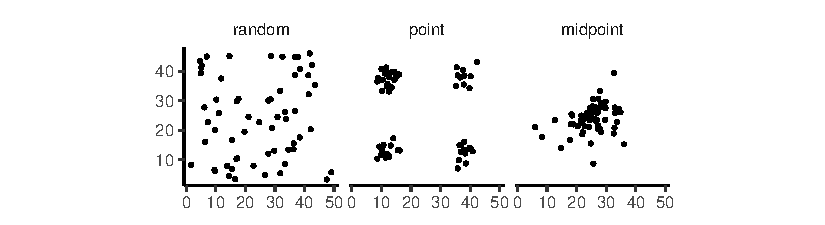
\includegraphics{figures/sampling_maps.pdf}
\caption{Example sampling maps for 60 individuals on a 50x50 landscape under midpoint, point, and random sampling strategies.}
\label{fig:samplemap}
\end{figure}

\begin{figure}[htbp]
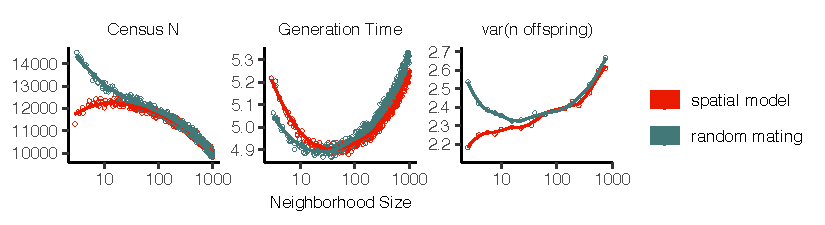
\includegraphics{figures/pop_params.pdf}
\caption{Genealogical parameters from spatial and random mating SLiM simulations, by neighborhood size.}
\label{fig:genparams}
\end{figure}


\begin{figure*}[p]
\centering
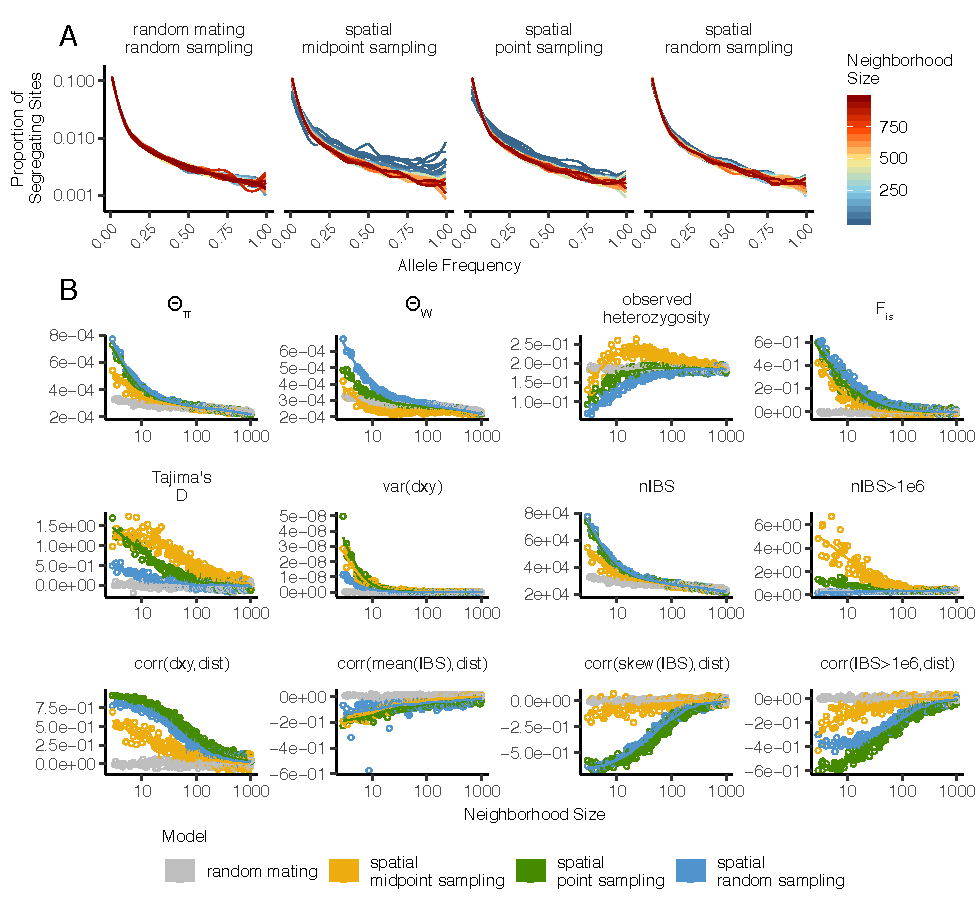
\includegraphics[width=\textwidth]{figures/sfs_w_sumstats.pdf}
\caption{A: Site frequency spectra under midpoint, point, and random sampling schemes. Lines are loess curves over the site frequency spectrum from each simulation with colors scaled to neighborhood size. Random mating models showed no differences by sampling scheme -- see supplementary figure S1. Spatial models have fewer low-frequency alleles and more mid-frequency alleles when neighborhood sizes are small, and this effect is stronger when sampling is more concentrated. B: Summary statistics under each sampling strategy, by neighborhood size.}
\label{fig:sumstats}
\end{figure*}

\afterpage{\clearpage}
\begin{figure*}[p]
\centering
\includegraphics[width=\textwidth]{figures/stairwayplot_facet_rollmean.pdf}
\caption{Inferred demographic histories for spatial SLiM simulations from Stairwayplot, by sampling scheme and neighborhood size (NS) range. The thick line is a rolling mean and thin lines are individual model fits. Dashed horizontal lines are the average $N_{e}$ across random-mating SLiM models estimated from $\theta_{\pi}$.}
\label{fig:demography}
\end{figure*}

\afterpage{\clearpage}
\begin{figure*}[p]
\centering
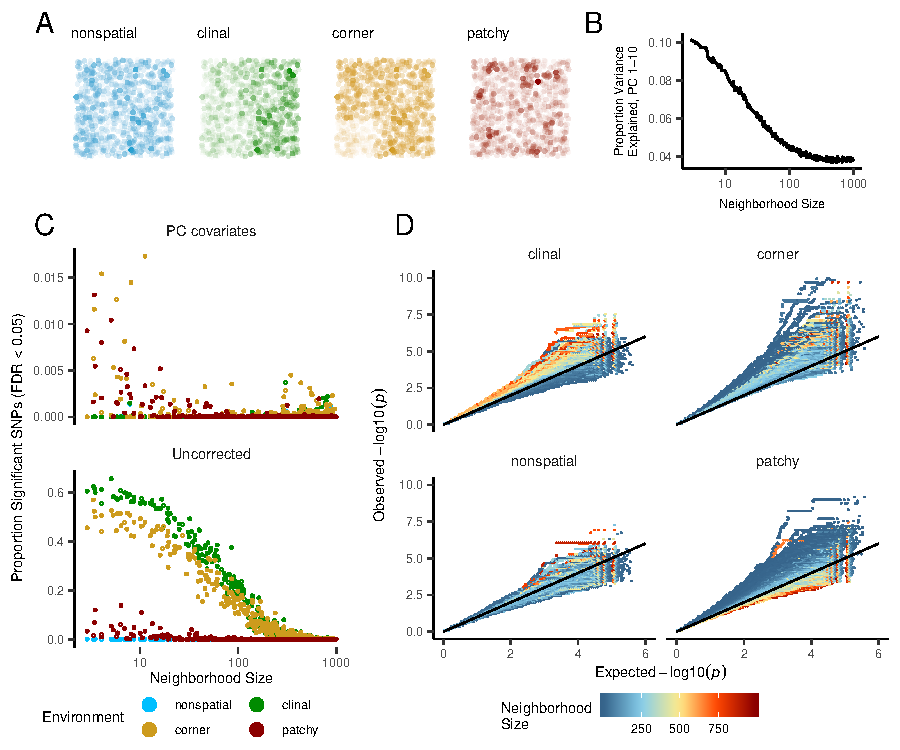
\includegraphics[width=\textwidth]{figures/gwas_summary.pdf}
\caption{Impacts of spatially correlated phenotypes and isolation by distance on linear regression GWAS.  A: example environmental distributions and sampling maps, with colors scaled to phenotype values. B: proportion of total variance explained by the first 10 PC axes, by neighborhood size. C: Proportion of significant SNPs after FDR correction for linear-model GWAS conducted with (top) or without (bottom) PC covariates, by neighborhood size. D: Quantile-quantile plots of observed $p$ values relative to those expected from a uniform distribution. The dotted lines show the 95\% confidence region assuming binomial sampling and an alpha level of 0.05. Points above the 1:1 line reflect deflated $p$ values.}
\label{fig:gwas}
\end{figure*}

\afterpage{\clearpage}
% latex table generated in R 3.5.1 by xtable 1.8-3 package
% Thu Apr 11 13:11:59 2019
\begin{table}[ht]
\centering
\caption{\bf Neighborhood size estimates from empirical studies. Survey methods indicate field studies to measure dispersal or population density. Genetic methods include both sequence-based analyses and enzyme activity assays or crosses used to estimate allele frequencies.}
\begin{tabular}{rllrrll}
  \hline
 Species & Description & \makecell[l]{Neighborhood\\Size} & Method & Citation \\ 
  \hline
  \makecell[l]{\textit{Ipomopsis}\\\textit{aggregata}} & flowering plant & 12.60 - 37.80 & Genetic & \citep{Campbell1992}\\
  \makecell[l]{\textit{Linanthus}\\\textit{parryae}} & flowering plant & 14 - 27 & Genetic & \citep{Wright1943}\\ 
  \makecell[l]{\textit{Borrichia}\\\textit{frutescens}} & salt marsh plant & 20 - 30 & Genetic+Survey & \citep{Antlfinger1982} \\ 
  \makecell[l]{\textit{Oreamnos}\\\textit{americanus}} & mountain goat & 36 - 100 & Genetic & \citep{Shirk2014} \\ 
  \makecell[l]{\textit{Homo sapiens}} & \makecell[l]{Gainj- and Kalam- \\speaking people,\\Papua New Guinea} & 40 - 213 & Genetic & \citep{Rousset1997}\\ 
  \makecell[l]{\textit{Formica sp.}} & colonial ants & 50 - 100 & Genetic & \citep{Pamilo1983} \\ 
  \makecell[l]{\textit{Astrocaryum}\\\textit{mexicanum}} & palm tree & 102 - 895 & Genetic+survey & \citep{Eguiarte1993} \\ 
  \makecell[l]{\textit{Spermophilus}\\\textit{mollis}} & ground squirrel & 204 - 480 & Genetic+Survey & \citep{Antolin2001}\\
  \makecell[l]{\textit{Sceloperus}\\\textit{olivaceus}} & lizard & 225 - 270 & Survey & \citep{Kerster1964} \\ 
  \makecell[l]{\textit{Dieffenbachia}\\\textit{longispatha}} & \makecell[l]{beetle-pollinated\\colonial herb} & 227 - 611 & Survey & \citep{Young1988} \\ 
  \makecell[l]{\textit{Homo sapiens}} & \makecell[l]{Gainj- and Kalam- \\speaking people,\\Papua New Guinea} & 410 & Survey & \citep{Rousset1997} \\ 
  \makecell[l]{\textit{Quercus}\\\textit{laevis}} & Oak tree & $>440$ & Genetic & \citep{Berg1995} \\ 
  \makecell[l]{\textit{Drosophila}\\\textit{pseudoobscura}} & fruit fly & 500 - 1,000 & Survey+Crosses & \citep{Wright1946} \\ 
  \makecell[l]{\textit{Homo sapiens}} & \makecell[l]{POPRES data\\NE Europe} & 1,342 - 5,425 & Genetic & \citep{Ringbauer2017} \\ 
  \makecell[l]{\textit{Bebicium}\\\textit{vittatum}} & intertidal snail & 240,000 & Survey & \citep{Rousset1997}\\ 
  \makecell[l]{\textit{Bebicium}\\\textit{vittatum}} & intertidal snail & 360,000 & Genetic & \citep{Rousset1997}\\ 
   \hline
\end{tabular}
\label{table:NStable}
\end{table}

\bibliography{spaceness}



%%%%%%%%%%%%%%%%%%%%%%%%%%%%%%%%%%%%%% Supplement %%%%%%%%%%%%%%%%%%%%%%%%%%%%%%%%%%%%%%%
\section{Supplementary Figures and Tables}
\beginsupplement

\afterpage{\clearpage}
\begin{figure*}[p]
\centering
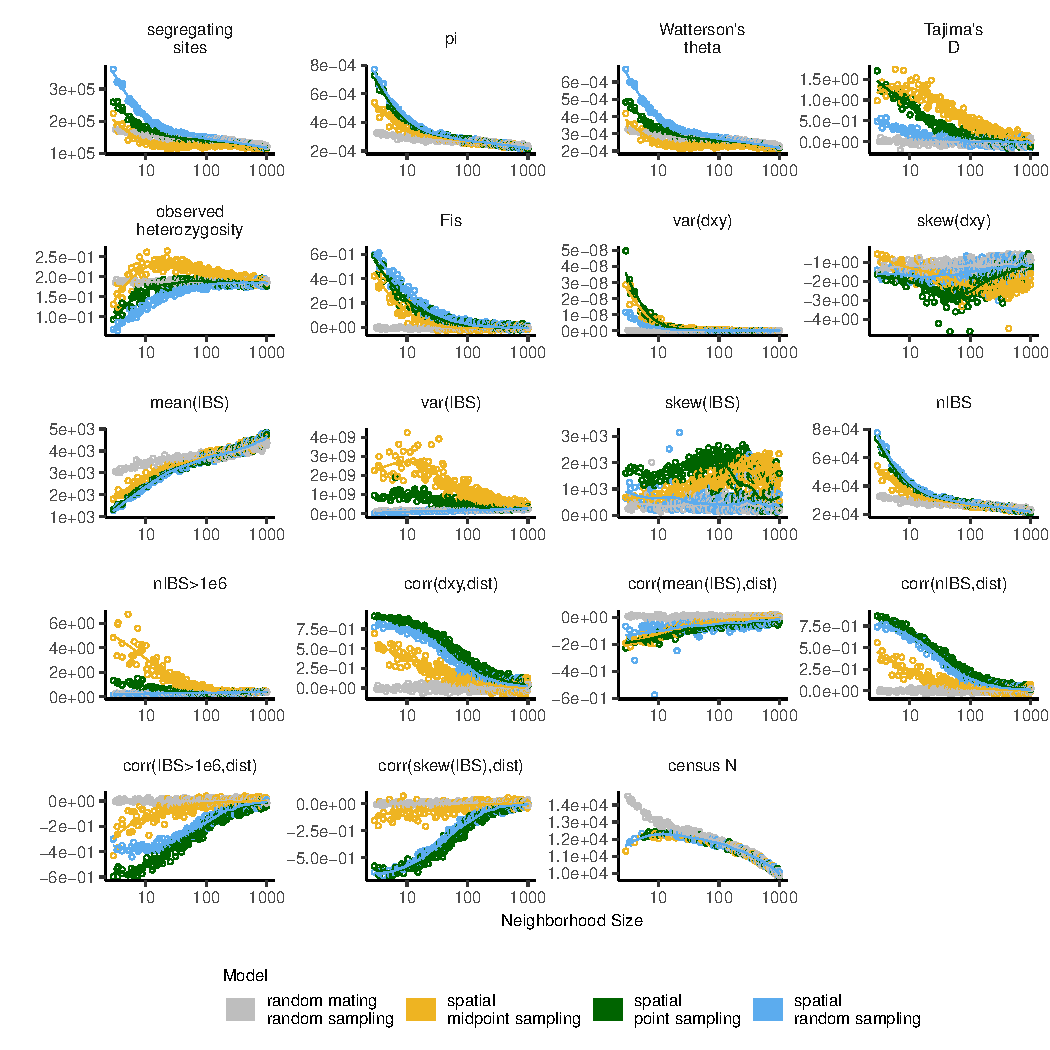
\includegraphics[width=\textwidth]{figures/sumstats_by_neighbors_allstats.pdf}
\caption{Change in summary statistics by neighborhood size and sampling scheme calculated from simulated sequence data of 60 individuals.}
\label{fig:allsumstats} 
\end{figure*}


\afterpage{\clearpage}
\begin{figure*}[p]
\centering
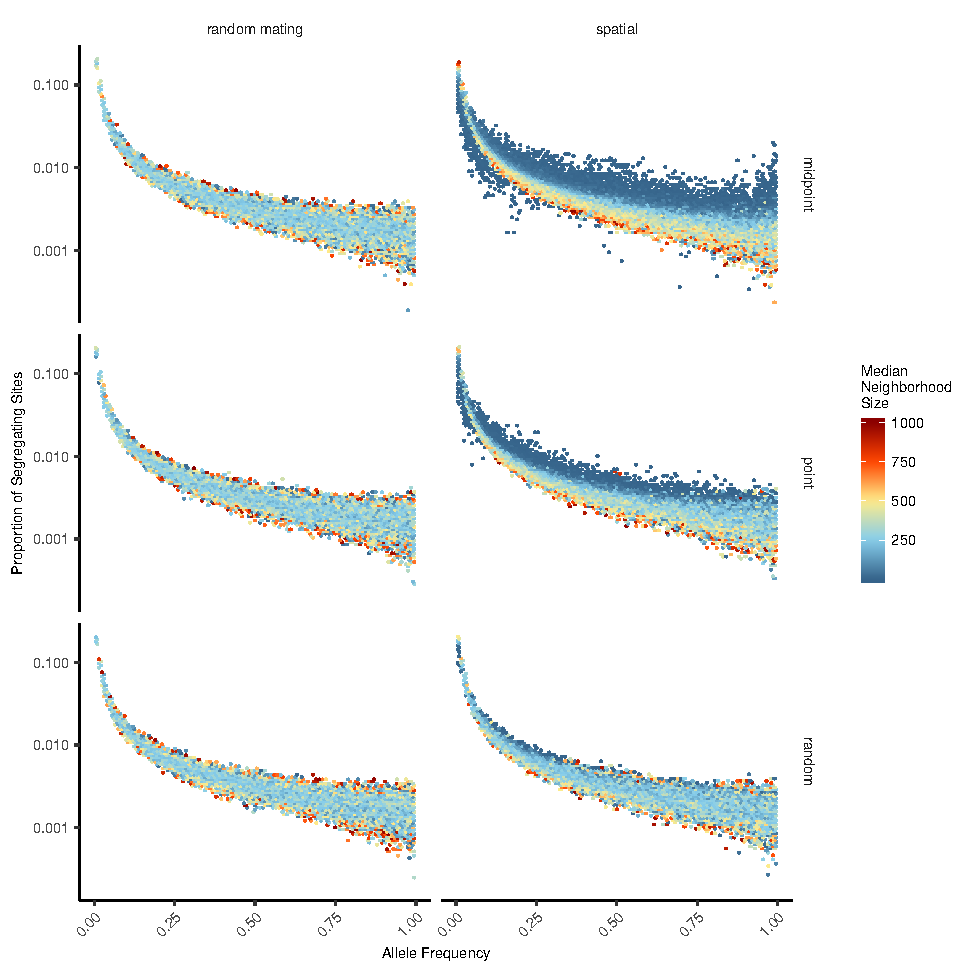
\includegraphics[width=\textwidth]{figures/fig_S1_sfs_grid_model_by_sampling.pdf}
\caption{Site frequency spectra for random mating and spatial SLiM models under all sampling schemes.}
\label{fig:allsfs}
\end{figure*}

\afterpage{\clearpage}
\begin{figure*}[p]
\centering
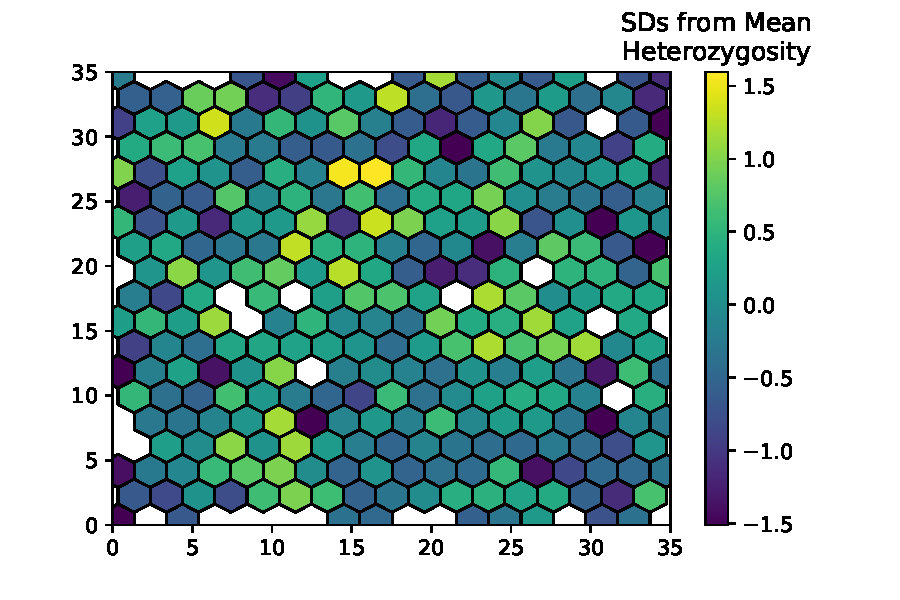
\includegraphics[]{figures/het_z_by_ind.pdf}
\caption{Normalized mean observed heterozygosity by location across 200 randomly-sampled individuals}
\label{fig:hetmap}
\end{figure*}

\begin{table*}[htbp]
\centering
\caption{\bf Anova and Levene's test $p$ values for differences by sampling strategy. Bolded values are rejected at \alpha=0.05}
\begin{tableminipage}{\textwidth}
\begin{tabularx}{\textwidth}{XXXX}
  \hline
 variable & model & p(equal means) & p(equal variance) \\ 
  \hline
segsites & random mating & 0.998190 & 0.980730 \\ 
pi & random mating & 0.997750 & 0.996450 \\ 
thetaW & random mating & 0.998190 & 0.980730 \\ 
tajD & random mating & 0.879690 & 0.188770 \\ 
het\_o & random mating & 0.531540 & 0.433230 \\ 
fis & random mating & 0.474790 & 0.785730 \\ 
gen\_dist\_mean & random mating & 0.997770 & 0.996510 \\ 
gen\_dist\_var & random mating & 0.283630 & 0.647240 \\ 
gen\_dist\_skew & random mating & 0.958320 & 0.260750 \\ 
gen\_sp\_corr & random mating & 0.601980 &\textbf{0.000000} \\ 
ibs\_mean & random mating & 0.997960 & 0.997730 \\ 
ibs\_var & random mating & 0.486450 & 0.399490 \\ 
ibs\_skew & random mating & 0.117980 & 0.069770 \\ 
ibs\_blocks\_per\_pair & random mating & 0.997680 & 0.996570 \\ 
ibs\_blocks\_over\_1e6\_per\_pair & random mating & 0.834870 & 0.888730 \\ 
ibs\_mean\_spat\_corr & random mating & 0.073270 & 0.308420 \\ 
ibs\_1e6blocks\_spat\_corr & random mating & 0.268440 & \textbf{0.002100} \\ 
ibs\_skew\_spat\_corr & random mating & 0.396920 & \textbf{0.000620} \\ 
ibs\_blocks\_spat\_corr & random mating & 0.581090 & \textbf{0.000000} \\ 
segsites & spatial & \textbf{0.000000} & \textbf{0.000000} \\ 
pi & spatial & \textbf{0.026510} & \textbf{0.013440} \\ 
thetaW & spatial & \textbf{0.000000} & \textbf{0.000000} \\ 
tajD & spatial & \textbf{0.000000} & \textbf{0.000000} \\ 
het\_o & spatial & \textbf{0.000000} & \textbf{0.000000} \\ 
fis & spatial & \textbf{0.000000} & \textbf{0.000120} \\ 
gen\_dist\_mean & spatial & \textbf{0.025390} & \textbf{0.012910} \\ 
gen\_dist\_var & spatial & \textbf{0.004970} & \textbf{0.006230} \\ 
gen\_dist\_skew & spatial & \textbf{0.000000} & \textbf{0.000000} \\ 
gen\_sp\_corr & spatial & \textbf{0.000000} & \textbf{0.000000} \\ 
ibs\_mean & spatial & 0.272400 & 0.114250 \\ 
ibs\_var & spatial & \textbf{0.000000} & \textbf{0.000000} \\ 
ibs\_skew & spatial & \textbf{0.000000} & \textbf{0.000000} \\ 
ibs\_blocks\_per\_pair & spatial & \textbf{0.033920} & \textbf{0.016640} \\ 
ibs\_blocks\_over\_1e6\_per\_pair & spatial & \textbf{0.000000} & \textbf{0.000000} \\ 
ibs\_mean\_spat\_corr & spatial & \textbf{0.000000} & 0.590540 \\ 
ibs\_1e6blocks\_spat\_corr & spatial & \textbf{0.000000} & \textbf{0.000000} \\ 
ibs\_skew\_spat\_corr & spatial & \textbf{0.000000} & \textbf{0.000000} \\ 
ibs\_blocks\_spat\_corr & spatial & \textbf{0.000000} & \textbf{0.000000} \\ 
\hline
\end{tabularx}
\end{tableminipage}
\label{table:sampling}
\end{table*}

% latex table generated in R 3.5.1 by xtable 1.8-3 package
% Fri Mar 22 13:50:47 2019
\begin{table}[ht]
\centering
\caption{\bf T-test results comparing standard deviations of inferred $N_{e}$ between spatial and coalescent models, by neighborhood size (NS) and sampling strategy. $p$ is the probability that spatial models have higher standard deviations.}
\begin{tabular}{rllrrrrr}
  \hline
sampling & NS range & t & df & $p$ \\ 
  \hline
random & 2-20 & 4.2572 & 41.6166 & 0.0001 \\ 
random & 20-100 & -1.8473 & 171.9905 & 0.9668 \\ 
random & 100-500 & -2.1297 & 164.3864  & 0.9827 \\ 
random & 500-1000 & -3.9681 & 147.0497 & 0.9999 \\ 
point & 2-20 & 7.0802 & 44.3615  & 0.0000 \\ 
point & 20-100 & -0.2038 & 169.3799 & 0.5806 \\ 
point & 100-500 & -2.4945 & 152.5000 & 0.9932 \\ 
point & 500-1000 & -3.8329 & 162.6443& 0.9999 \\ 
midpoint & 2-20 & 5.9253 & 59.5462 & 0.0000 \\ 
midpoint & 20-100 & 3.8940 & 171.7005  & 0.0001 \\ 
midpoint & 100-500 & -2.2764 & 139.5221 & 0.9878 \\ 
midpoint & 500-1000 & -3.2223 & 165.0792 & 0.9992 \\ 
   \hline
\end{tabular}
\label{table:demography}
\end{table}


\stopsupplement



\end{document}

